\chapter{player charges}
\label{sec:charges}
\lhead[tempest]{}
\lstset{style=6502Style}

\begin{figure}[H]
    \centering
    \begin{adjustbox}{width=11cm,center}
      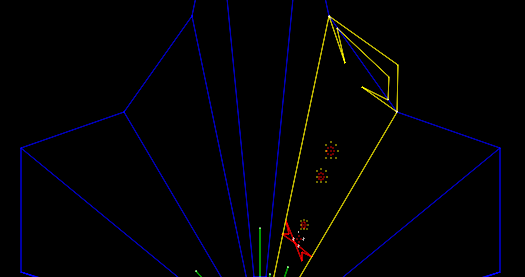
\includegraphics[width=12cm]{src/bullets/bullets.png}%
    \end{adjustbox}
  \caption*{Cursor Firing Charges, or as we like to call them: Bullets.}
\end{figure}

For some reason, the player's bullets in \textit{TEMPEST}, are referred to as 'charges'.
When fired they run along the rail the player occupies, into the well in the hope of striking
an unwitting alien. Let's take a look at how we get these charges on to the screen.

\begin{minipage}[c]{0.58\linewidth}
\begin{figure}[H]
    \centering
    \begin{adjustbox}{width=8cm,center}
      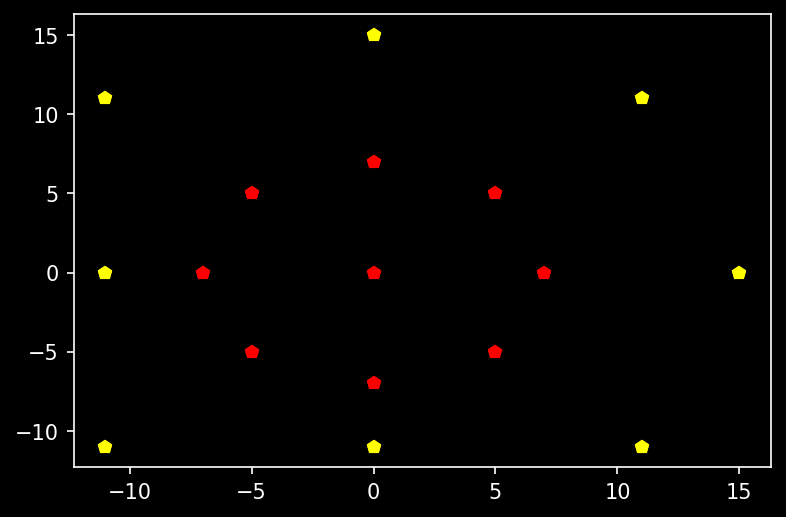
\includegraphics[width=12cm]{src/bullets/red_bullet.png}%
    \end{adjustbox}
    \caption*{The bullet as drawn by \icode{DIARA2} opposite.}
\end{figure}
\end{minipage}
\hspace{0.5cm}
\begin{minipage}[c]{0.35\linewidth}
  \begin{lstlisting}[basicstyle=\scriptsize\ttfamily]
DIARA2: ICVEC
        CSTAT PSHCTR
        SCDOT 0,0
        SCDOT 7,0
        SCDOT 5,5
        SCDOT 0,7
        SCDOT -5,5
        SCDOT -7,0
        SCDOT -5,-5
        SCDOT 0,-7
        SCDOT 5,-5
        CSTAT YELLOW
        SCDOT 0F,0
        SCDOT 0B,0B
        SCDOT 0,0F
        SCDOT -0B,0B
        SCDOT -0B,0
        SCDOT -0B,-0B
        SCDOT 0,-0B
        SCDOT 0B,-0B
        RTSL
\end{lstlisting}
\vspace*{\fill}
\end{minipage}

We draw the charges at a given point in time by keeping a list of their depth in
the well in \icode{CHARY} (short for \icode{CHARGES Y POSITION}). This means
that drawing them is as simple as looping through this list and drawing any
entry that has a non-zero depth value.

\begin{lstlisting}
        .SBTTL  DISPLAY-CHARGES
        ; THIS ROUTINE WILL LOOP THROUGH ALL THE CHARGES
        ; AND DRAW ANY OF THEM THAT ARE ACTIVE.
DSPCHG:
        LDX I,NCHARG-1  ; GET THE NUMBER OF CHARGES (IT'S 8).
        STX INDEX1      ; STORE IT AS OUR INDEX.

        ; LOOP THROUGH ALL 8 CHARGES (BULLETS) AND DRAW
        ; ANY THAT ARE ACTIVE.
        BEGIN           ; START OF LOOP
        LDX INDEX1      ; GET CURRENT INDEX AND USE IT TO..
        LDA X,CHARY     ; ..GET THE VALUE IN THE CURRENT SLOT.
        IFNE            ; IS IT ACTIVE?
        STA PYL         ; IF YES, SCAPIC EXPECTS THE DEPTH IN PYL.
        LDY X,CHARL1    ; GET THE LINE THE BULLET IS ON.
        LDA I,PTCURS    ; GET THE PICTURE IN DIARA2.
        JSR SCAPIC      ; DRAW THE BULLET USING THE VALUES ABOVE.
        ENDIF
        DEC INDEX1      ; DECREMENT OUR INDEX..
        MIEND           ; AND LOOP AGAIN IF STILL NOT ZERO.

        ; SET THE COLOR OF THE CENTRE OF THE BULLET TO INDICATE
        ; HOW MANY SHOTS ARE AVAILABLE TO THE PLAYER.
        LDY I,ZYELLO    ; BY DEFAULT, YELLOW INDICATES PLENTY.
        LDA CHACOU      ; GET THE NO. OF BULLETS CURRENTLY IN PLAY.
        CMP I,NPCHARG-2 ; IF BETWEEN 6 AND 8..
        IFCS            ; THEN IT'S 'LOW' SO..
        LDY I,ZBLUE     ; SET COLOR TO BLUE ('LOW').
        CMP I,NPCHARG   ; IF IT'S 8...
        IFCS            ; THEN THERE ARE NO MORE LEFT..
        LDY I,ZRED      ; SET COLOR TO RED ('OUT').
        ENDIF
        ENDIF
        ; SET THE COLOR WE CHOSE FOR CENTER OF BULLET.
        STY COLPOR+PSHCTR     ; NOTICE PSHCTR IS REF'D BY DIARA2 ABOVE.
        RTS
\end{lstlisting}

There is a little-noticed subtlety in how we draw the bullets in the code above. Since
there are eight bullets available to the player at any one time, we colour-code the bullets
according to how many are currently in play. If all eight bullets are currently in play, we
will colour them red. If there are between 5 and 7, we colour them blue. Otherwise we colour
them all yellow. Personally I'd never realized this was happening until I read the code!

\begin{figure}[H]
  {
    \setlength{\tabcolsep}{3.0pt}
    \setlength\cmidrulewidth{\heavyrulewidth} % Make cmidrule = 
    \begin{adjustbox}{width=15cm,center}
      \begin{subfigure}{0.3\textwidth}
        \begin{figure}[H]
          \centering
          \begin{adjustbox}{width=4cm,center}
            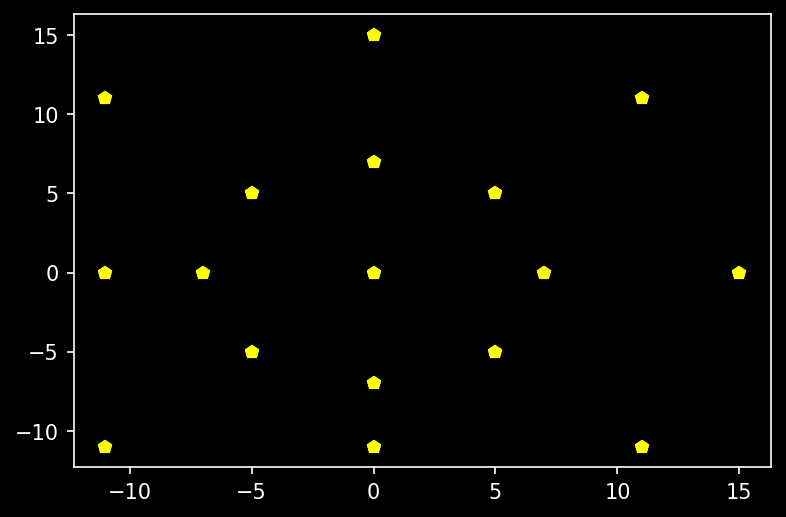
\includegraphics[width=12cm]{src/bullets/yellow_graph.png}%
          \end{adjustbox}
          \caption{YELLOW: \icode{PLENTY}}
        \end{figure}
      \end{subfigure}
      \begin{subfigure}{0.3\textwidth}
        \begin{figure}[H]
          \centering
          \begin{adjustbox}{width=4cm,center}
            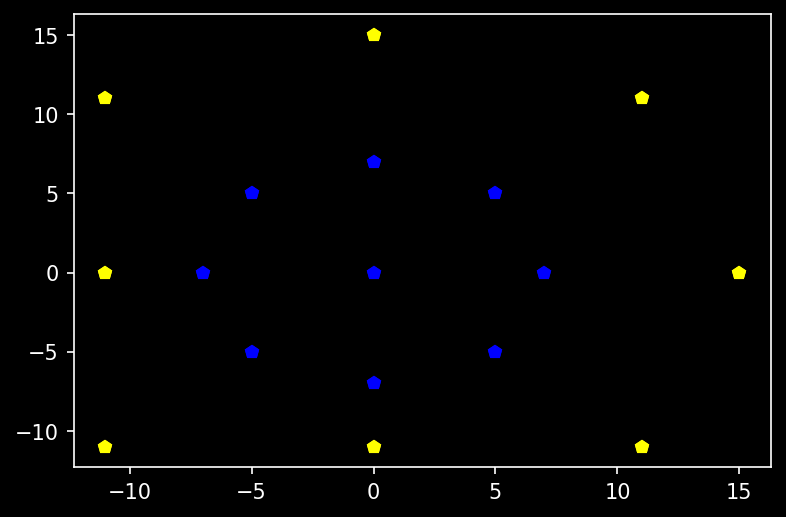
\includegraphics[width=12cm]{src/bullets/blue_graph.png}%
          \end{adjustbox}
          \caption{BLUE: \icode{LOW}}
        \end{figure}
      \end{subfigure}
      \begin{subfigure}{0.3\textwidth}
        \begin{figure}[H]
          \centering
          \begin{adjustbox}{width=4cm,center}
            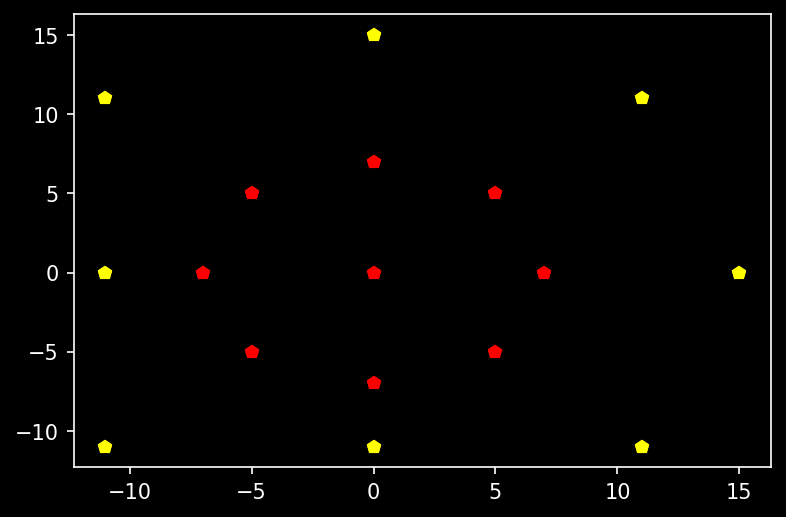
\includegraphics[width=12cm]{src/bullets/red_graph.png}%
          \end{adjustbox}
          \caption{RED: \icode{OUT}}
        \end{figure}
      \end{subfigure}
    \end{adjustbox}
    }\caption[]{Different colours of the bullets depending on how many shots are left.}
\end{figure}

The actual drawing to the screen of each bullet is worth pausing over. First of all, what
do we want to do? We want to draw each bullet a little further along the line it was originally
fired on. This means that we have to pick a position that is a combination of horizontal (\icode{X}),
vertical (\icode{Z}), and depth (\icode{Y}) points and draw the bullet centred at that point.

You may have noticed that we were using the list of 'depth' points (\icode{CHARY}) to decide whether or not
to draw a bullet in the first place, so we already have the depth value we want to draw at stored in
\icode{PYL}. This leaves the vertical and horizontal positions. To retrieve this for a particular bullet
we used a list called \icode{CHARL1} that stores the line that each bullet belongs to. Armed with this
'line number' in the \icode{Y} register the first part of our drawing routine (\icode{SCAPIC}), we can
use it to get the appropriate horizontal and vertical position for that line from a pair of special
tables. Now that we have all three points we can draw the bullet in its position. 

\clearpage
\begin{lstlisting}
;FUNCTION: DISPLAY A PICTURE CENTERED BETWEEN 2 POINTS AND SCALED
;          DOWN ACCORDING TO ITS DEPTH
;INPUT: X = INDEX INTO LINEX,Z OF 1ST PT'S X & Z WC WORDS
;       Y = INDEX INTO LINEX,Z OF 2ND PT'S X & Z WC WORDS
;       COLOR=COLOR OF OBJECT
;       PYL = Y WC COORD FOR BOTH PTS.
;       ACC = CODE FOR PICTURE TO DISPLAY (INDEX INTO PICLO)
SCAPIC:
        STA OBJIND        ; STORE THE PICTURE INDEX IN OBJIND
        LDA Y,LINEXM      ; GET THE X COORD. OF MIDWAY PT.
        STA PXL           ; STORE IN PXL
        LDA Y,LINEZM      ; GET THE Z COORD OF MIDWAYPT.
        STA PZL           ; STORE IN PZL
    
        ; USE PXL,PYL, AND PZL TO CALCULATE THE CENTRE POINT FOR
        ; THE BULLET ON THE SCREEN. THE RESULT IS STORED IN
        ; SXL AND SZL. THEN MOVE THE BEAM TO THE DESIRED POSITION
        ; BY ADDING SOME OPCODE INSTRUCTION TO THE VECTOR GENERATOR
        ; LIST.
        JSR WORSCR        ; CALCULATE SXL AND SZL.
        LDX I,SXL         ; GET THE CALCULATED CENTRE PT.
        JSR VGYAB1        ; DRAW A BLANK VECTOR TO IT SO WE START THERE.
    
        ; CALCULATE THE SCALE AND ADD IT AS AN OPCODE TO THE VGLIST.
        LDA I,0           ; VGY IS OUR INDEX INTO THE VGLIST..
        STA VGY           ; ..SO SET IT TO 0 SO WE'RE AT THE START.
        JSR CASCAL        ; CALCULATE SCALE
    
        ; CALCULATE THE BRIGHTNESS AND ADD IT AS AN OPCODE TO THE VGLIST.
        LDA BFACTR        ; GET THE BRIGHTNESS FACTOR.
        EOR I,7
        ASL
        CMP I,0A
        IFCC
        LDA I,0A
        ENDIF
        ASL
        ASL
        ASL
        ASL
        STA NY,VGLIST     ; STORE THE BRIGHTNESS BYTE
        INY               ; MOVE TO NEXT BYTE OF OPCODE
        LDA I,60          ; '60' IS THE ID OF THE BRIGHTNESS OPCODE.
        STA NY,VGLIST     ; STORE THE ID IN THE OPCODE LIST.
        INY               ; INCREMENT THE INDEX.
        STY VGY           ; STORE IT.
    
        ; ADD THE OPCODE TO THE VGLIST FOR DRAWING THE BULLET.
        LDY OBJIND        ; GET THE INDEX OF THE BULLET PIC.
        LDX Y,PICHI       ; GET THE HI BYTE OF THE BULLET PIC.
        LDA Y,PICLO       ; GET THE LO BYTE OF THE BULLET PIC.
        LDY VGY           ; GET THE CURRENT INDEX IN THE OPCODE LIST.
        JMP VGADD3        ; DRAW PIC AT PT.
\end{lstlisting}
So the result of a typical visit to the \icode{SCAPIC} routine is to generate 
a series of Op-Codes that are added to the Vector Generator list. The first set
is generated by calling \icode{VGYAB1} and
is responsible for moving the beam to the desired position on screen.
\begin{figure}[H]
  {
    \setlength{\tabcolsep}{3.0pt}
    \setlength\cmidrulewidth{\heavyrulewidth} % Make cmidrule = 
    \begin{adjustbox}{center}
      \begin{tabular}[t]{lll}
        \toprule
        Vector Commands & Command Meaning & Result on Screen\\

        \midrule
          \icode{7100}
        &
        \makecell[tl]{
          \begingroup
          \renewcommand{\arraystretch}{.8} % Default value: 1
          \begin{tabular}[t]{ll}
            Set Scale: & \icode{00}\\
            \icode{} &  \\
          \end{tabular}
          \endgroup
        } &
        \multirow{3}{*}[-0.1cm]{
          \makecell[tl]{
            
\includegraphics[height=2.1cm]{bullets/blank.png}%
          }
        } \\
        \addlinespace
          \icode{8040}
        &
        \makecell[tl]{
          \begingroup
          \renewcommand{\arraystretch}{.8} % Default value: 1
          \begin{tabular}[t]{ll}
            Move to Center\\
          \end{tabular}
          \endgroup
        } &
        \\
        \addlinespace
          \icode{1F2AE4AB}
        &
        \makecell[tl]{
          \begingroup
          \renewcommand{\arraystretch}{.8} % Default value: 1
          \begin{tabular}[t]{ll}
            Draw Relative Vector: & \icode{}  \\
            \icode{} &  \\
          \end{tabular}
          \endgroup
        } &
        \\

        \bottomrule
      \end{tabular}
    \end{adjustbox}
  }
\end{figure}
We follow that by setting the scale again, then the brightness, and finally
drawing the bullet itself.
\begin{figure}[H]
  {
    \setlength{\tabcolsep}{3.0pt}
    \setlength\cmidrulewidth{\heavyrulewidth} % Make cmidrule = 
    \begin{adjustbox}{center}
      \begin{tabular}[t]{lll}
        \toprule
        Vector Commands & Command Meaning & Result on Screen\\

        \midrule
          \icode{7308}
        &
        \makecell[tl]{
          \begingroup
          \renewcommand{\arraystretch}{.8} % Default value: 1
          \begin{tabular}[t]{ll}
            Set Scale: & \icode{308}\\
            \icode{} &  \\
          \end{tabular}
          \endgroup
        } &
        \multirow{3}{*}[-0.1cm]{
          \makecell[tl]{
            
\includegraphics[height=2.3cm]{bullets/bullet.png}%
          }
        } \\
        \addlinespace
          \icode{680A}
        &
        \makecell[tl]{
          \begingroup
          \renewcommand{\arraystretch}{.8} % Default value: 1
          \begin{tabular}[t]{ll}
            New Color: & Not Set\\
            Intensity: &  \icode{0A}\\
          \end{tabular}
          \endgroup
        } &
        \\
        \addlinespace
          \icode{AFA7}
        &
        \makecell[tl]{
          \begingroup
          \renewcommand{\arraystretch}{.8} % Default value: 1
          \begin{tabular}[t]{ll}
            Jump to Routine: & \icode{DIARA2}  \\
            \icode{} &  \\
          \end{tabular}
          \endgroup
        } &
        \\

        \bottomrule
      \end{tabular}
    \end{adjustbox}
  }
\end{figure}

%\begin{lstlisting}
%        .SBTTL PLAY - FIRE PLAYER CHARGE
%FIREPC:
%        LDA CURSL2
%        IFPL                    ;PLAYER ALIVE
%        LDA QSTATUS
%        IFPL                    ;ATTRACT?
%        LDA CURMOD              ;YES. AUTO FIRE
%        STA TEMP0
%        LDX I,NICHARG+NINVAD-1
%        BEGIN                   ;LOOP FOR EACH INVADER & SHOT UNTIL EXHAUSTED OR CLOSE 1 IS FOUND
%        LDA X,CHARY+NPCHAR
%        IFNE                    ;ACTIVE?
%        LDA X,CHARL1+NPCHAR     ;YES CALUCLATE ABSOLUTE VALUE OF LINE DELTA
%        SEC                     ;
%        SBC CURSL1
%        IFMI
%        EOR I,0FF
%        CLC
%        ADC I,1
%        ENDIF
%        CMP I,2
%        IFCC                    ;TOO CLOSE?
%        INC TEMP0               ;YES. FIRE
%        ENDIF
%        ENDIF
%        DEX
%        MIEND
%        LDA TEMP0
%        ELSE
%        LDA SWSTAT
%        AND I,MFIRE
%        ENDIF
%        IFNE                    ;FIRE CHARGE?
%        LDX I,NPCHARG-1         ;YES
%        BEGIN                   ;LOOP UNTIL VACANCY IS FOUND
%        LDA X,CHARY
%        IFEQ                    ;VACANCY?
%                                ;YES FIRE CHARGE
%        INC CHACOU
%        LDA CURSY               ;START AT CURSOR
%        STA X,CHARY
%        LDA CURSL1
%        STA X,CHARL1            ;STARTS AT SAME LINE AS CURSOR
%        LDA CURSL2
%        STA X,CHARL2
%        LDA I,0                 ;0 COLLISION COUNTER
%        STA X,CHARCO
%        JSR SLAUNC              ;LAUNCH SOUND
%        LDA CURSY
%        JSR COLCHK              ;CHECK FOR COLLISION
%        LDX I,0                 ;EXIT LOOP
%        ENDIF
%        DEX
%        MIEND
%        ENDIF
%        ENDIF
%        RTS
%\end{lstlisting}
%Now thatWhen the player presses fire, we must decide whether or not to actually fire a bullet.
%This is because there can only be 8 bullets in play at once. 
%\begin{lstlisting}
%NPCHARG=8
%        .SBTTL PLAY - FIRE PLAYER CHARGE
%FIREPC:
%        ..
%        LDX I,NPCHARG-1                ;YES
%        BEGIN                        ;LOOP UNTIL VACANCY IS FOUND
%        LDA X,CHARY
%        IFEQ                        ;VACANCY?
%                                ;YES FIRE CHARGE
%        INC CHACOU
%        LDA CURSY                ;START AT CURSOR
%        STA X,CHARY
%        LDA CURSL1
%        STA X,CHARL1                ;STARTS AT SAME LINE AS CURSOR
%        LDA CURSL2
%        STA X,CHARL2
%        LDA I,0                        ;0 COLLISION COUNTER
%        STA X,CHARCO
%        JSR SLAUNC                ;LAUNCH SOUND
%        LDA CURSY
%        JSR COLCHK                ;CHECK FOR COLLISION
%        LDX I,0                        ;EXIT LOOP
%        ENDIF
%\end{lstlisting}
